\chapter{Machine learning in natural language processing} \label{Machine learning in natural language processing}

- General pipeline 5p
- Ulmfit, bert, electra 10p

What to write about:
- Simple preprocessing tasks such as manual data cleaning, data quality improvements
- Tokenization and data representation with topics such as n-grams, language modeling, embeddings (word2vec) and word/sentencepiece tokenization
- Modern (BERT/ULMFit/ELECTRA) way of training models: pretraining, finetuning with a notion to transfer learning
- Evaluation metrics

- 3.1


This chapter first gives an overview of the parts of a general machine learning pipeline and then describes the methodology of three modern machine learning models: ULMFit, BERT and ELECTRA.

\section{Transfer learning} \label{Transfer learning}
Transfer learning refers to the ability of a system to reuse knowledge learned in a previous task in a task of new or novel domain that shares some commonality with the previous task \cite{yang2020}.
Often the motivation for using transfer learning comes from a lack of labelled training data for a specific task.
In natural language processing it is widely used to first teach a model on a general language corpus, so that it learns the generalities of the given language, and then fine-tuning the model on some downstream task, such as classification.

All of the introduced NLP-models later in this chapter use transfer learning as each has a clear distinction between the pre-training and finetuning phases in model training where another model's pre-trained state can be transferred to another task and finetuned further for that task.


\subsection{Embeddings} \label{Embeddings}
The tranferral of knowledge can be achieved by many means.
A common case in NLP has been to use word embeddings that encode some information about a word in relation to other words in the feature space.
Using embeddings is a general way of transferring knowledge as it doesn't depend on any specific model architecture but only on the language used.
The most popular methods for generating vector representations for words have been Word2Vec \cite{mikolov2013}, GLoVe \cite{pennington2014}, and fastText \cite{bojanowski2017}, all of which will be presented in the next sections.

\subsubsection{Word2Vec} \label{Word2Vec}
Word2Vec is an open-source project based on the work by Mikolov et al. that can be used to train distributed representations of words and phrases \cite{mikolov2013}.

\begin{figure}[t]
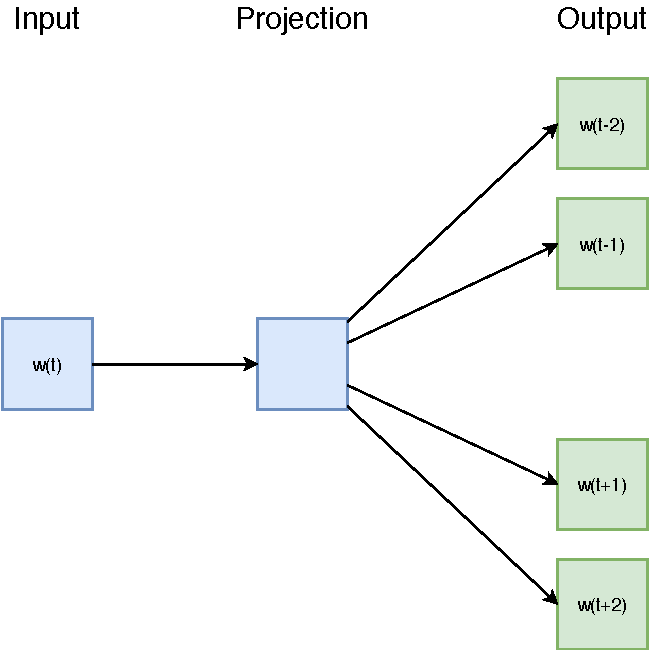
\includegraphics[scale=0.6]{skipgram}
\centering
\caption{Skip-gram model architecture.}
\label{fig:skipgram}
\end{figure}

It uses a skip-gram model (figure \ref{fig:skipgram}), proposed by Mikolov et al. in an earlier work \cite{mikolov2013a}, that is a prediction-based method.
The training objective of the skip-gram model is to find useful word representations for predicting the surrounding words in a sentence or a document.
It learns these representation by predicting the surrounding words for each word in a sentence within a defined max distance from the word.
Mikolov et al. show, that the produced representations exhibit linear structure that makes precise analogical reasoning possible \cite{mikolov2013}.

Given the computationally efficient model architecture of the skip-gram, the training times of Word2Vec are manageable even with huge amounts of data.

\subsubsection{GLoVe} \label{GLoVe}
Global Vectors for Word Representation (GLoVe) is a model to construct word representations.
It is a global log-bilinear regression model that combines the advantages from both Word2Vec-style local context window methods and global matrix factorization.
Training of GLoVe is done on aggregated global word-word co-occurrence statistics \cite{pennington2014}.

Given the same corpus and equal compute, Pennington et al. show that it outperforms Word2Vec and achieves better results faster \cite{pennington2014}, although Levy et al. \cite{levy2015} came to the opposite conclusion after careful testing.

\subsubsection{fastText} \label{fastText}
fastText is an open-source library for learning word embeddings and text classification.
It builds on the work of Word2Vec and improves on the skip-gram model by incorporating character n-grams in it.
Words are now represented as a sum of n-gram vectors instead of a single vector.
This is especially important for morphologically rich languages, such as Finnish, that contain many word forms that occur rarely in the training corpus, which makes learning good word representations difficult \cite{bojanowski2017}.

Mikolov et al. show that fastText significantly outperforms GLoVe on a number of tasks \cite{mikolov2017}.

\subsection{Language modeling}\label{Language modeling}
-- TALK ABOUT HOW LM IS CURRENTLY THE WAY TRANSFER LEARNING IS GENERALLY USED IN DEEP LEARNING NLP --


\section{Preprocessing} \label{Preprocessing}
Before a machine learning model can be trained, the data for it has to be gathered and preprocessed.
Preprocessing in NLP usually consists of a number of steps such as lemmatization and tokenization.

This section describes common steps used in preprocessing in NLP.

\subsection{Tokenization} \label{Tokenization}
\cite{webster1992}
\subsubsection{SentencePiece} \label{SentencePiece}

SentencePiece is a subword tokenizer and detokenizer that is language independent and designed for machine learning -based processing. \cite{kudo2018}
Compared to other subword segmentation systems, SentencePiece does not require that the input is pre-tokenized into word sequences. It works natively with raw sentences thus allowing a purely language independent and end-to-end system.

SentencePiece's language-independent quality is quite important especially for Neural Machine Translation (NMT), which can perform automatic translation with a simple end-to-end system. Numerous NMT-systems rely on language dependent pre- and post-processors. Adding sentencepiece to those systems simplifies the processing pipeline and removes the need for custom processors for different languages.

SentencePiece is comprised of four different components: Normalizer, Trainer, Encoder and Decoder. \cite{kudo2018} Normalizer is used to transform semantically equivalent characters to a canonical form. The Trainer trains a subword segmentation model from the normalized corpus. The Encoder first normalizes the text with the Normalizer and encodes raw text into a subword sequence using the model generated by the Trainer. The Decoder can be used to transform the tokens into normalized text. \cite{kudo2018}

Compared to whole word tokenization, SentencePiece's subword tokenization achieves a lossless representation of data. For example, a traditional tokenizer might tokenize "Hello world." as [Hello][World][.], thus losing the information of where there are spaces in the sentence. SentencePiece treats whitespace as a normal symbol and replaces all occurrences of whitespace with an underscore (U+2581) before tokenization. SentencePiece might tokenize the aforementioned example as [Hello][\_wor][ld][.] thus preserving the whitespace.\cite{kudo2018}

SentencePiece builds a vocabulary of a predefined size of subword tokens. Depending on the given maximum size, the subwords' length changes. If, for example, the given maximum size is just 30 or so, the vocabulary could consist of all the letters of the english alphabet and not much else. On the other hand, if the vocabulary is excessively large, it would essentially work like a normal whole word tokenizer. Thus, the maximum vocab size becomes another tunable hyperparameter, which has a considerable impact on model performance.

Given the abundance of inflections in the Finnish language, one would think that SentencePiece could work better for preprocessing it than other alternatives such as spaCy, which tokenizes and numericalizes whole words instead of subwords.

\subsubsection{Other tokenizers} \label{Other tokenizers}

\subsection{Lemmatisation}\label{Lemmatisation}



\section{Training} \label{Training}

\subsection{Pretraining and finetuning} \label{Pretraining and finetuning}
\subsection{Methods} \label{Methods}

\subsubsection{SGD}

\subsubsection{}


\section{Architectures} \label{Architectures}

\subsection{RNN} \label{RNN}
\begin{figure}[t]
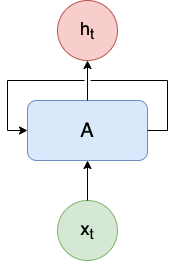
\includegraphics[scale=0.7]{rnnloop}
\centering
\caption{An RNN-module which illustrates the recurrent nature of the model}
\label{fig:rnnloop}
\end{figure}

Recurrent neural networks (RNN) are networks that process an input sequence one token at a time and maintain a state in its hidden units that contains information about the past elements in the sequence.
This approach has been proven to work well with tasks that contain sequential input such as speech, language and music \cite{lecun2015}.
Figure \ref{fig:rnnloop} shows the basic methodology behind an RNN: a chunk of neural network, A, looks at the input $x_t$ and ouputs a value $h_t$. The output value is looped back as a second input value which allows for information to be passed from one step to the other.

Figure \ref{fig:rnn} shows a visualization of the insides of an RNN module which is quite simple in practice. $x_t$ represents an input at timestep $t$, $tanh$ is a function that returns the hyperbolic tangent of the input and $h_t$ is the hidden state of the network at timestep $t$.
First the hidden state from the previous timestep and the current input value are added to each other after which the sum is fed into the $tanh$ function.
$tanh$ essentially squishes the input value between -1 and 1 to keep the values from exploding due to repeated multiplication.
The output of tanh is the new hidden state, the memory of the network, which is then fed to the next timestep.

\begin{figure}[t]
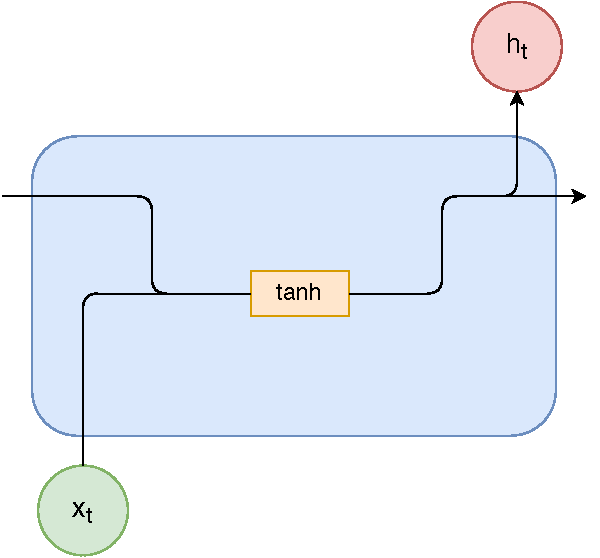
\includegraphics[scale=0.4]{rnn}
\centering
\caption{An unrolled RNN}
\label{fig:rnn}
\end{figure}

The training of an RNN happens by using a variant of backpropagation called \textit{backpropagation through time} (bptt) which is a generalization of backpropagation for networks which store the activations of units while going forward in time \cite{rumelhart1985}.
The backward gradient update pass is thus also backward in time and recursively computes the required gradients with the saved activations.
It is easy to see how this works when the different timesteps of an RNN are unrolled and displayed as if they combine to make a single neural network with multiple layers (fig \ref{fig:rnn}).

RNNs have difficulties maintaining long-term dependencies when processing lengthy input sequences that originates from the \textit{vanishing gradients} problem \cite{bengio1994}:
During backpropagation gradients, with which the weights of the network are updated, change as they are applied backwards through time.
A small change to a layer before means an even smaller change in the current layer.
On the contrary, gradients with big changes tend to "blow up".
This means that the earlier layers in the network either stop learning since they only receive small gradient updates or their weights oscillate due to big changes \cite{hochreiter1997}.
In an RNN this problem is magnified due to backpropagation being applied to each time step.

\subsection{LSTM} \label{LSTM}
Long short-term memory (LSTM) is a recurrent network architecture proposed by Hochreiter and Schmidhuber in 1997 \cite{hochreiter1997}.
LSTM was designed to combat the vanishing gradients problem that is especially prevalent in RNNs.
LSTMs work exceptionally well on a large variety of problems and are widely used nowadays.

Figure \ref{fig:lstm} illustrates an lstm module. Each line carries a vector, merging lines denote concatenation, forking lines denote copying of the vector and each copy going to different directions, orange boxes are learned neural network layers and purple circles represent pointwise operations such as multiplication, addition and hyperbolic tangent.
In addition to keeping track of the hidden state of the network, LSTM adds another state called cell state that is denoted by the horizontal line running through the top of the figure.
Information is added and removed to the cell state by gates that are made up of sigmoid ($\sigma$) neural net layers and pointwise multiplication operations.
A sigmoid neural net layer takes as input the concatenation of the previous hidden state $h_{t-1}$ and the current input $x_t$ and outpus a vector of values between 0 and 1 to describe how much of each value is to be let through.
A value of 1 lets everything through while a 0 lets nothing through.
An LSTM has three of these gates.
From left to right, the first gate forms the forget gate layer which decides what data to keep and what to discard from the previous cell state.
Next, the data to add to the cell state is decided with a combination of a $sigmoid$ layer and a $tanh$ layer. The $tanh$ layer outputs new candidate values and the $sigmoid$ layer decides which of them to add to the cell state.
Finally, the last layer determines the output (hidden state) of the cell by taking the current cell state's values and applying a $tanh$ function to push the values between -1 and 1 and multiplying them with the output of the $sigmoid$ gate.
The new cell state and hidden state are then passed on to the next time step.
\begin{figure}[t]
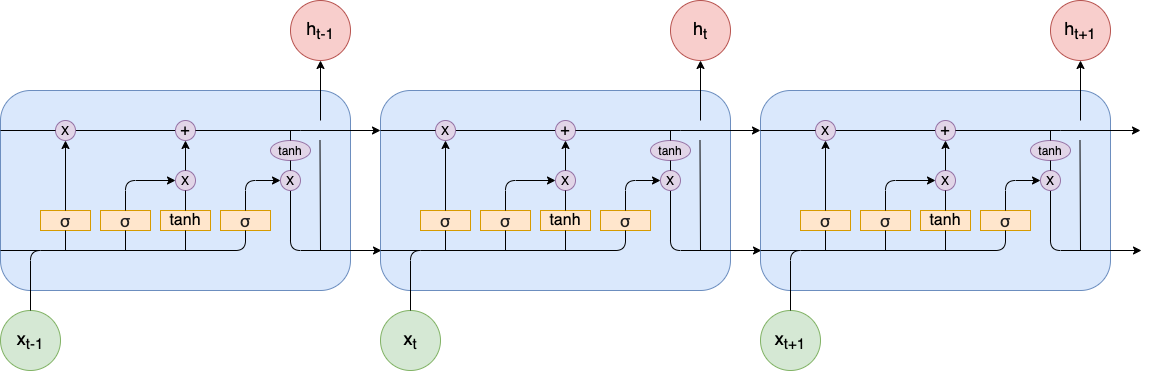
\includegraphics[scale=0.4]{lstm}
\centering
\caption{Long short-term memory network}
\label{fig:lstm}
\end{figure}

The LSTM architecture described above is considered a standard version of LSTM, but other variants exist too.
One popular variant of LSTM introduced by Gers \& Schmidhuber \cite{gers2000a} adds peephole-connections that allow the gate layers to look at the cell state.
Another variant called the \textbf{Gated Recurrent Unit} (GRU, figure \ref{fig:gru}), introduced by Cho, et al. \cite{cho2014}, simplifies the model by combining the forget and input gates into a single update gate.
\begin{figure}[t]
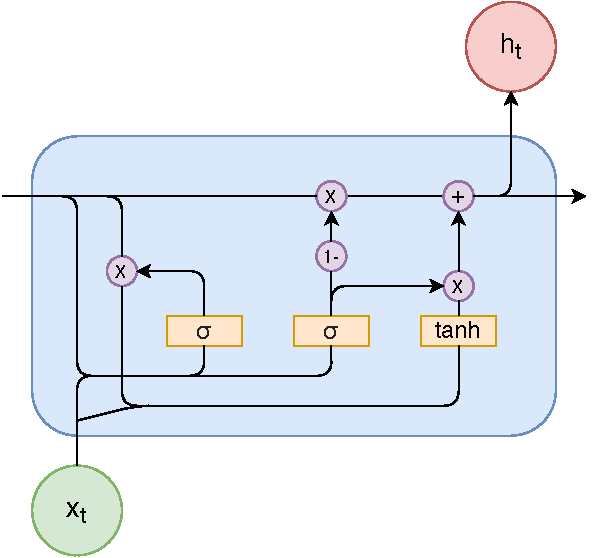
\includegraphics[scale=0.4]{gru}
\centering
\caption{Gated Recurrent Unit}
\label{fig:gru}
\end{figure}

\subsection{Transformer} \label{Transformer}
RNNs, as presented before, are inherently sequential in nature.
They take an input at timestep $t$ and compute a hidden state $h_t$ with knowledge from the previous hidden state $h_{t-1}$.
This sequentiality prohibits efficient parallelization within training examples since one has to come before the other in training.
Parallelization across examples is also critically constrained by memory at longer sequence lengths.
In addition to this, RNNs suffer from the so-called \textit{vanishing gradient problem} which is exacerbated at longer sequence lengths.
\cite{vaswani2017}

Attention is a mechanism that allows the modeling of dependencies without regard for distance in input or output sequences.
It has been used in conjunction with recurrent neural networks to achieve good results, but using it with RNNs somewhat limits the power of attention since the model is still constrained by the aforementioned problems of RNNs.
Thus Vaswani et al. proposed a novel architecture in 2017, the Transformer, in the paper \textit{Attention is all you need}, to combat these limitations.
The Transformer has been the foundation of neural networks that have achieved state-of-the-art results in various language-related tasks in the last couple of years \cite{vaswani2017}.

The Transformer consists of an encoder, which maps an input sequence of tokens to a sequence of continuous representations, and a decoder, which takes a continuous representation and generates an ouput sequence.
The output sequence is generated one token at a time while taking the previous generated tokens as additional input.

\begin{figure}[t]
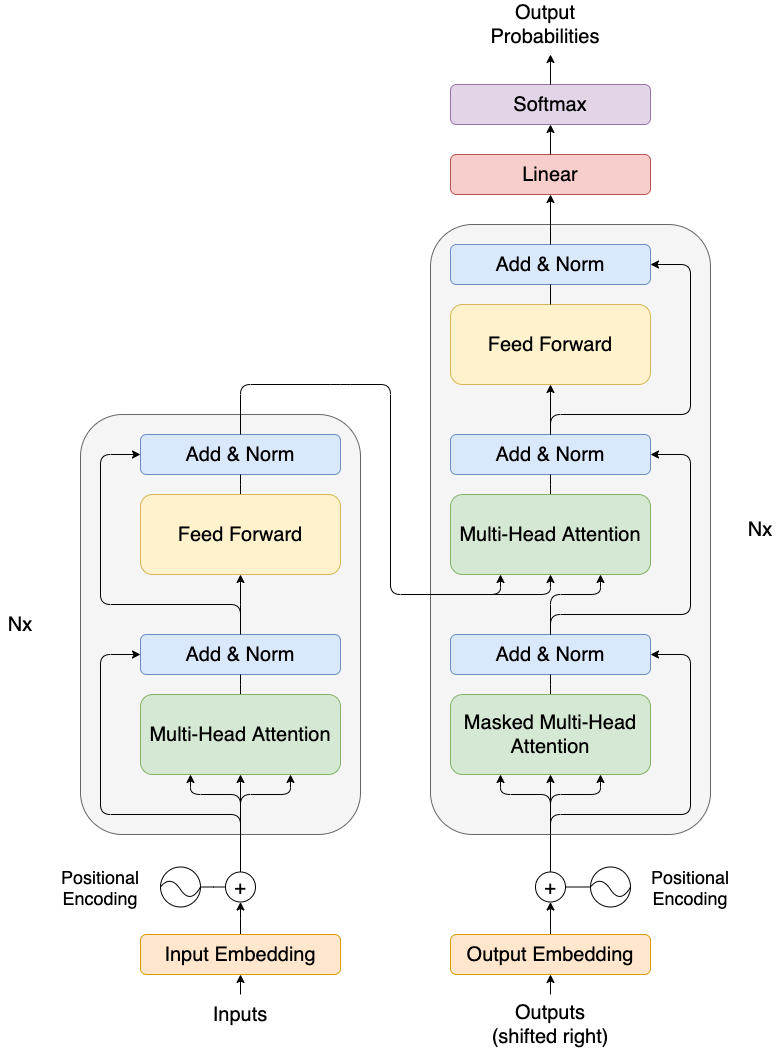
\includegraphics[scale=0.4]{transformer}
\centering
\caption{The Transformer, from the paper \textit{Attention is all you need} \cite{vaswani2017}}
\label{fig:transformer}
\end{figure}

The overall architecture of the Transformer is shown in Figure \ref{fig:transformer}, with the left side of the figure representing the encoder and the right side the decoder.
The encoder is composed of six identical layers stacked on top of each other.
Each layer consists of two sub-layers; a multi-head self-attention mechanism and a fully connected feed-forward network.
Residual connections \cite{he2016} are used around each sub-layer to shortcut the sub-layers while training.
This leads to faster training times and a more robust model as the connections are gradually restored during training.
Finally, layer normalization is applied to the output of the sub-layer as $LayerNorm(x+Sublayer(x))$, where $Sublayer(x)$ refers to the function implemented by the sub-layer.
Due to the residual connections, all sub-layers and embedding layers have to produce outputs of the same dimension.
Thus in the Transformer the dimension is defined as $d_{model}=512$.

The decoder is also composed of six identical layers but additionally includes a third sub-layer, which applies multi-head attention over the output of the encoder stack.
The self-attention sub-layer in the decoder stack is also modified to prevent positions from attending to subsequent positions.
Thus predictions for position $i$ can only depend on the outputs before $i$.

Attention can be described as a function of mapping a query and a set of key-value pairs to an output \cite{vaswani2017}.
The query, keys, values and output are all vectors.
The output is a weighted sum of the values, where the weight of each value is defined by a compatibility function of the query with the corresponding key.
The particular version of attention in the Transformer is called \textit{Scaled Dot-Product Attention} in which the input consists of queries and keys of dimension $d_k$ and values of dimension $d_v$.
The dot products of queries with all keys are computed first, denoted by $QK^T$ in equation \ref{eq:attention}.
The results are divided by $\sqrt{d_k}$ and then a softmax function is applied to obtain the weights on the values.


\begin{equation}
  Attention(Q,K,V)=softmax(\dfrac{{QK^T}}{{\sqrt{d_k}}})V\label{eq:attention}
\end{equation}

Instead of using a single attention function over all the keys, values and queries with dimension $d_{model}$, the Transformer uses so-called \textit{Multi-Head Attention} to linearly project the keys, values and queries $h$ times to $d_k$, $d_k$ and $d_v$ dimensions.
The attention function is then applied in parallel to all these projected versions, yielding $d_v$-dimensional outputs.
These outputs are then concatenated and projected to achieve the final result.
This allows the model to jointly attend to information from different representation subspaces at different positions \cite{vaswani2017}.
In the Transformer, 8 parallel attention heads are used.

Attention is used in three different ways in the Transformer.
In encoder-decoder attention, where the output of the encoder is used in the decoder, the queries come from the previous decoder layer and the keys and values come from the output of the encoder, and in encoder and decoder self-attention.
In encoder self-attention all the queries, keys and values come from the output of the previous encoder layer, thus each position in the encoder can attend to all positions in the previous encoder layer.
Decoder self-attention similarly receives its input from the previous decoder layer's output, but doesn't allow attention over all the positions but only up to and including the current position.
This is achieved by masking out all the input values of the softmax corresponding to illegal connections.

The decision to use self-attention was made based on three requirements: to minimize the total computational complexity of each layer, to maximize the amount of parallelizable computation and to minimize the path length between long-range dependencies.
A side benefit of self-attention is more interpretable models as attention distributions can be inspected and tested with different examples to gain insight into the behaviour of individual attention heads \cite{vaswani2017}.

\subsection{Other architectures} \label{Other architectures}
-- AUTOENCODER --
-- CNN --

\section{Evaluation} \label{Evaluation}

\subsection{Tasks}\label{Tasks}

\subsection{Measures} \label{Measures}

\subsubsection{Accuracy} \label{Accuracy}
Accuracy is the fraction of correctly classified documents in relation to the total number of documents.

\subsubsection{Precision} \label{Precision}

\begin{equation}
  \dfrac{\#\{relevant \cap retrieved\}}{\#retrieved}
\end{equation}

\subsubsection{Recall} \label{Recall}

\begin{equation}
  \dfrac{\#\{relevant \cap retrieved\}}{\#relevant}
\end{equation}

\subsubsection{F-score} \label{F-score}

\begin{equation}
  F=\dfrac{2}{1/recall + 1/precision}
\end{equation}

\section{Modern models} \label{Modern models}

\subsection{ULMFiT} \label{ULMFiT}
Universal Language Model Finetuning (ULMFiT) is a transfer learning based methodology for text classification which posted state-of-the-art results when it was published in 2018.
It consists of firstly pretraining a language model on a general-domain corpus and then finetuning it on a classification task.
This idea of first pretraining on a large general corpus and then finetuning it has been tried before, but has proven to be a challenging task due to it requiring millions of in-domain documents to achieve good performance \cite{dai2015}.
With ULMFiT Howard et al. proposed novel training techniques to make the training feasible even with a small corpus \cite{howard2018}.

ULMFiT is a \textit{universal} method in that it uses a single architecture and training process, requires no custom feature engineering, works across tasks with variable document sizes and label types, and doesn't require additional in-domain documents or labels \cite{howard2018}.

ULMFiT uses a 3-layer weight-dropped long shot-term memory (AWD-LSTM) network, proposed by Merity et al. \cite{merity2017}, which is a recurrent neural network (RNN).
AWD-LSTM is a vanilla LSTM with various regularization and optimization strategies such as DropConnect \cite{wan}, which prevents overfitting by randomly dropping connections between the recurrent hidden to hidden weight matrices, and averaged gradient descent as its optimization algorithm.

The training begins with pretraining a general-domain language model with unlabeled text data to capture the general properties of language.
This initial training step is the most expensive in the whole method but only needs to be done once.

After the general language model is trained, it is finetuned with the target task data.
This finetuning converges faster than the initial pretraining since the model needs to only adapt to the idiosyncrasies of the finetuning data.
This allows the training of robust language models even with small datasets.
ULMFiT uses \textit{discriminative fine-tuning} and \textit{slanted triangular learning rates} for the finetuning step of the language model.
With discriminative fine-tuning, instead of using a single learning rate for all the layers in the model, each layer is fine-tuned with a learning rate of its own.
The motivation for this comes from the fact that different layers capture different types of information, thus each layer should be fine-tuned for different amounts.
With slanted triangular learning rates, the learning rate is first linearly increased in order to get the model to quickly converge to a suitable region, and then linearly decreased to refine its parameters.

For the final step, two additional linear blocks are added to the end of the network, and the final classifier is fine-tuned with \textit{gradual unfreezing}.
Gradual unfreezing is used to prevent \textit{catastrophic forgetting} by unfreezing the layers of the model one by one, starting from the last.
Unfrozen layers are fine-tuned for one epoch after which the next layer is unfrozen until all the layers of the model have been unfrozen.
The whole model is then fine-tuned until convergence \cite{howard2018}.

Although outshined by BERT and other huge transformer-based models, ULMFiT is much fast to train and doesn't require a lot of data to get good results.




\subsection{BERT} \label{BERT}
Bidirectional Encoder Representations from Transformers (BERT) is a language representation model based on the Transformer \cite{vaswani2017} architecture (subsection \ref{Transformer}).
It uses a \textit{fine-tuning} based approach, in which all the pretrained parameters are finetuned when applying pre-trained language representations to down-stream tasks, as opposed to a \textit{feature-based} approach, where the pre-trained representations are only used as additional features in a task-specific architecture.

Both the fine-tuning and feature-based approach share the same objective function during pre-training of learning general language representations by using unidirectional language models.
BERT uses a \textit{masked language model} (MLM) pre-training objective to achieve bidirectionality in context, thus allowing the model to see both left and right of the input token when training.
MLM randomly masks tokens in the input, and the objective is to predict the vocabulary id of the masked token based on its context.
BERT also uses a \textit{next sentence prediction} (NSP) task that jointly pre-trains text-pair representations \cite{devlin2019}.

As with ULMFiT, BERT also has a unified architecture across different tasks with a minimal difference between the pre-trained architecture and the final downstream one.
BERT's architecture is almost identical with the Transformer described in section \ref{Transformer}, the difference comes mainly in the number of layers (Transformer blocks), denoted as $L$, hidden size, denoted as $H$ and the number of attention heads, denoted as $A$.
Results for BERT performace was primarily reported for two sizes: $BERT_{BASE}$ (L=12, H=768, A=12, total parameters=110M) and $BERT_{LARGE}$ (L=24, H=1024, A=16, total parameters=340M).

BERT uses WordPiece embeddings \cite{wu2016}, essentially similar to SentencePiece embeddings (section \ref{SentencePiece}).
Pre-training happens by the two aforementioned unsupervised tasks: Masked language modeling and next sentence prediction.

In MLM, 15\% of all WordPiece tokens are randomly chosen and each chosen token has an 80\% chance to actually be masked, a 10\% chance to be replaced with a random token, and a 10\% chacne to stay unchanged.
The reason for not always masking the chosen tokens is because the [MASK] token does not appear during fine-tuning, causing a mismatch between the two steps otherwise.

In NSP, training examples consist of two sentences $A$ and $B$.
50\% of the time $B$ is actually the next sentence that follows $A$ (label $IsNext$) and 50\% of the time its a random sentence from the corpus (label $NotNext$).

With the use of the Transformer-architecture, WordPiece embeddings and two pre-training objectives that allow bidirectional context, BERT was able to exceed the state-of-the-art on multiple downstream tasks.

\subsection{ELECTRA} \label{ELECTRA}
Efficiently Learning an Encoder that Classifies Token Replacements Accurately (ELECTRA) is a further elaboration on the BERT model by Clark, et al. \cite{clark2020}
The primary motivation for ELECTRA is making pretraining more efficient given that training a full-sized BERT or any derivation of it (ALBERT, RoBERTa etc.) requires a considerable amount of compute and training data.
As described in the BERT chapter (chapter \ref{BERT}), BERT uses masked language modeling as a pretraining objective.
This MLM is inherently quite inefficient in it's usage of the training data; only the masked tokens, approximately 15\% of the data, needs to be predicted.
As an alternative, ELECTRA proposes \textit{replaces token detection}, a pretraining task in which the model has to predict whether or not a token is the original token in the corpus or if it has been swapped for a token generated by a small masked language model.
This also solves the mismatch in BERT where the model sees [MASK] tokens during pretraining but not during finetuning.
ELECTRA trains the network as a discriminator rather than a generator, since it is predicting whether an input is corrupted or not.
This way ELECTRA learns from all the input tokens, rather than a small subset of them.

ELECTRA substantially outperforms MLM-based methods given the same amount of data and compute and works well even with relatively small amounts of compute \cite{clark2020}.
